\documentclass{beamer}
\usepackage{multicol,lipsum,caption}
\usepackage{amsmath,booktabs,verbatim,tikz}
\usepackage{biblatex}
\addbibresource{NAS.bib}
\usetikzlibrary{shapes.geometric, arrows,positioning,matrix,calc}
%\usepackage{mathptmx}

\usetheme[progressbar=frametitle]{metropolis}
\setbeamertemplate{frame numbering}[fraction]
\useoutertheme{metropolis}
\useinnertheme{metropolis}
\usefonttheme{metropolis}
\usecolortheme{spruce}
\setbeamercolor{background canvas}{bg=white}

\title{Neural Architecture Design}
\author{Huiyao ang}
\institute{Kyoto Institue of Technology}
\date{06-01-2020}


\begin{document}

\begin{frame}
    \titlepage
\end{frame}

\begin{frame}[c]{Content} 
    Original Ideas
    \begin{enumerate}
        \item Building Blocks of Neural Network 
        \item Multiple Transfer Functions  dsdsd
    \end{enumerate}
\end{frame}

\begin{frame}{Evolutionary Design of ANN}
    \begin{center}
          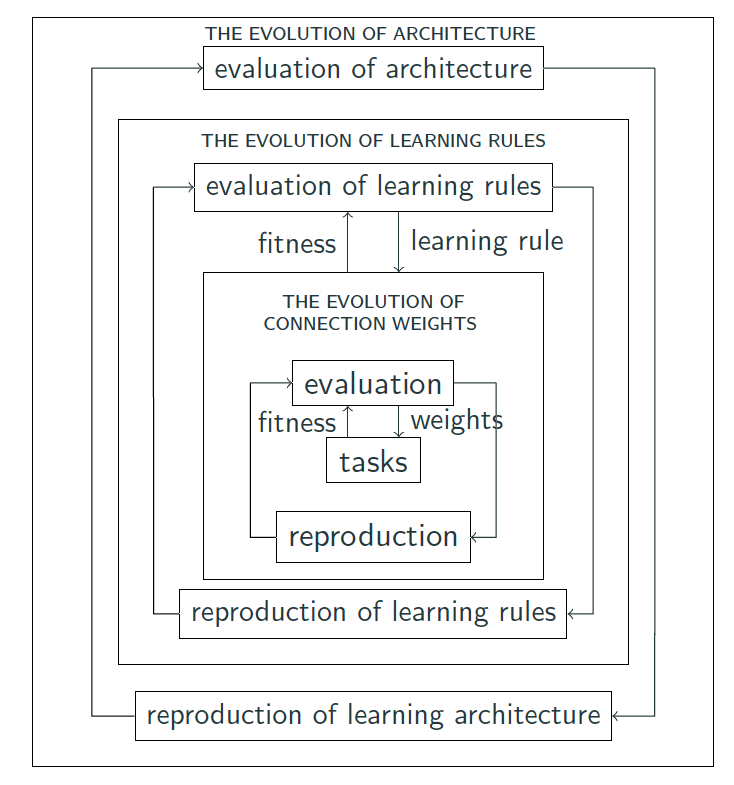
\includegraphics[scale=0.22]{NAS/general-architecture.png}
          \captionof{figure}{General Search Architecture}
    \end{center}
    \footfullcite{miller1989designing}
\end{frame}

\begin{frame}{Building Blocks}
    \begin{columns}[c]
    \begin{column}{0.5\textwidth}
        \begin{center}
              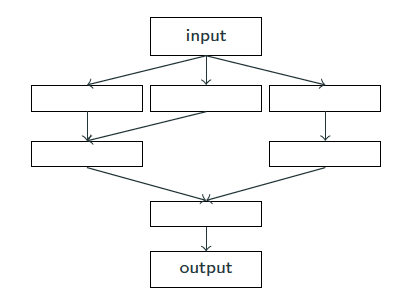
\includegraphics[width=0.9\linewidth]{NAS/cell-1.png}
              \captionof{figure}{Normal Cell}
        \end{center}
    \end{column}
    \begin{column}{0.5\textwidth}
        \begin{center}
              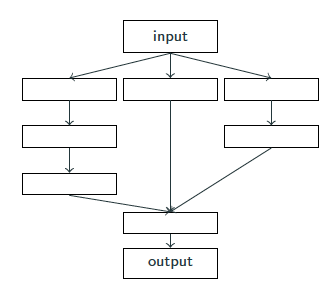
\includegraphics[width=0.8\linewidth]{NAS/cell-2.png}
              \captionof{figure}{Reduction Cell}
        \end{center}
    \end{column}
\end{columns}

\footfullcite{zoph2016neural}
\end{frame}
\begin{frame}{Stack Method}
    \begin{center}
        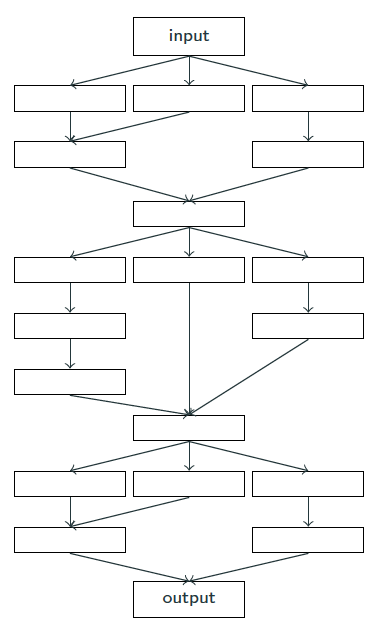
\includegraphics[scale=0.27]{NAS/chained-nerual-net.png}
          \captionof{figure}{Chained Neural Network}
    \end{center}
    \footfullcite{elsken2018neural}
\end{frame}



\begin{frame}{Stack Method}
    \begin{center}
          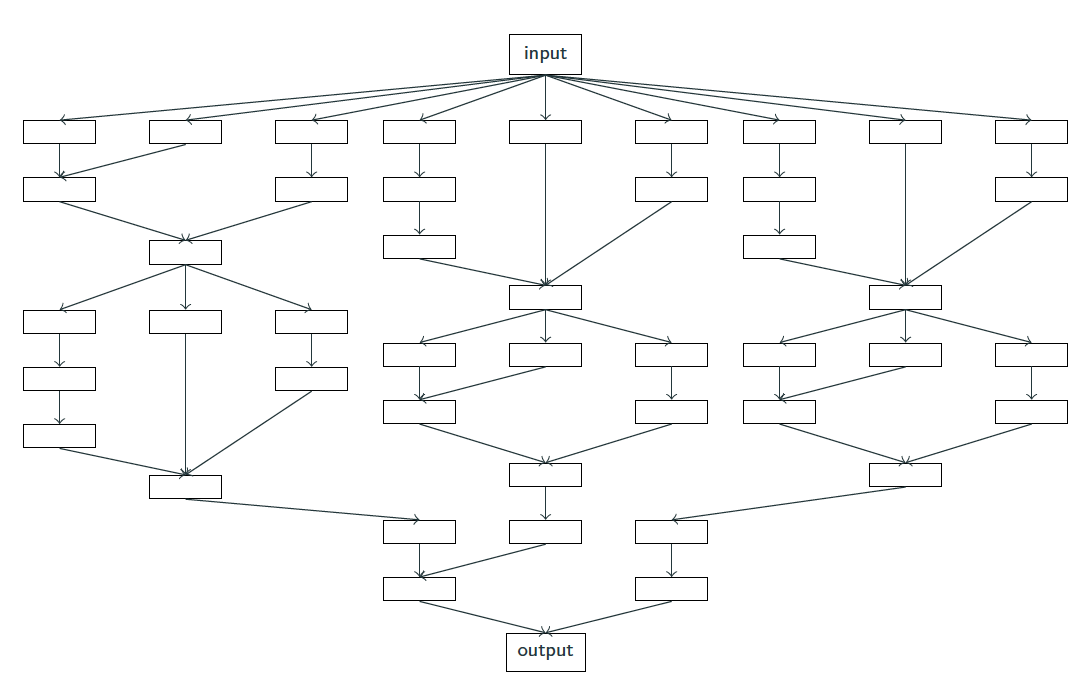
\includegraphics[width=0.8\linewidth]{NAS/multibranch-neural-net.png}
          \captionof{figure}{Multi-branch Neural Network}
    \end{center}
\end{frame}



\begin{frame}{Transfer Function}
    \begin{enumerate}
        \item Sigmoid
            \begin{equation}
                f(x)=\frac{1}{1+e^{-\beta x}}
            \end{equation}
        \item Piecewise Linear
            \begin{equation}
                f(x)=\left\{\begin{array}{ll}0 & \text { if } x \leq x_{\min }
                        \\ m x+b & \text { if } x_{\max }>x>x_{\min } \\ 1 &
                    \text { if } x \geq x_{\max }\end{array}\right.
                    \end{equation}
        \item Gaussian
            \begin{equation}
                f(x)=\frac{1}{\sqrt{2 \pi \sigma}} e^{\frac{-(x-\mu)^{2}}{2
                \sigma^{2}}}
            \end{equation}

    \end{enumerate}
    \footfullcite{liu1996evolutionary}
\end{frame}

\begin{frame}{Hybrid Training}
    \begin{columns}[c]
    \begin{column}{0.5\textwidth}
        \begin{enumerate}
            \item GA: Global Optimization
            \item BP: Local Optimization asds
        \end{enumerate}
    \end{column}
    \begin{column}{0.7\textwidth}
        \begin{center}
              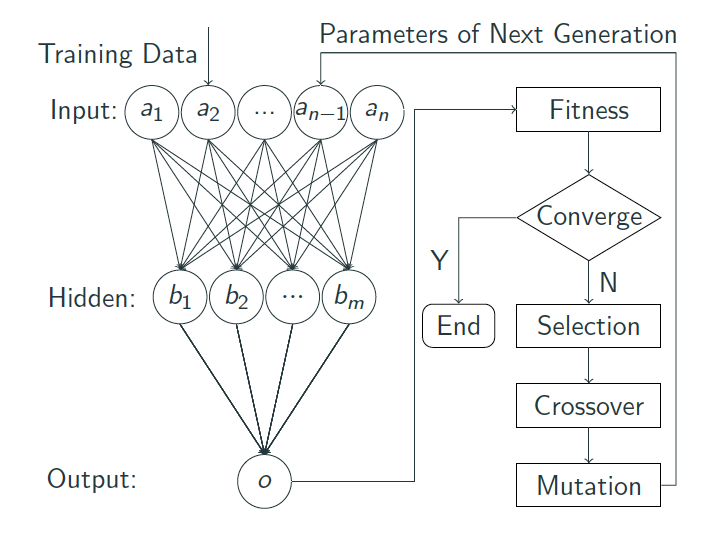
\includegraphics[scale=0.3]{NAS/hybrid-training.png}
              \captionof{figure}{Hybrid Training}
        \end{center}
    \end{column}
\end{columns}
\end{frame}

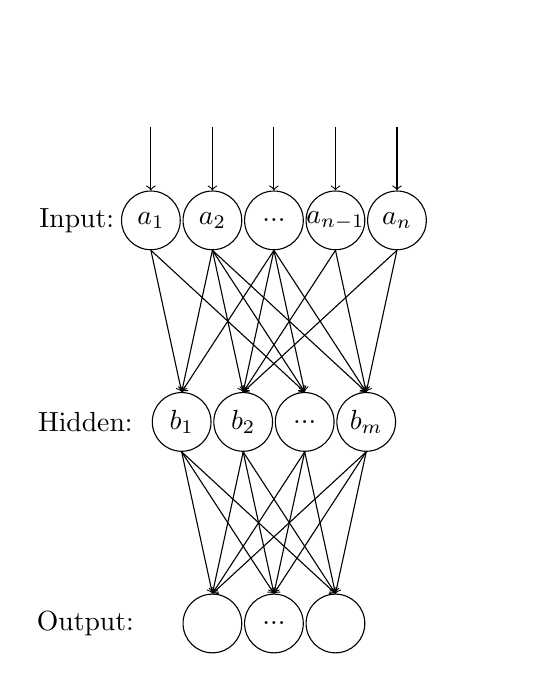
\begin{tikzpicture}
[ plain/.style={ draw=none, fill=none, }, remember picture, net/.style={ matrix of nodes, nodes={ draw, circle,
    inner sep=7.5pt
    },
  nodes in empty cells,
  column sep=-10.5pt,
  row sep=1.8cm
  }
]
    \draw[white] (2,4) rectangle (3,5);
%\draw[help lines] (-3cm,-6cm) grid (6cm,3cm);
\matrix[net] (mat)
{
              & |[plain]| &           & |[plain]|  &           & |[plain]| &           &  |[plain]|      &               \\
    |[plain]| &           & |[plain]| &            & |[plain]| &           & |[plain]| &                 & |[plain]|     \\ 
    |[plain]| & |[plain]| &           & |[plain]|  &           & |[plain]| & 	  	   &  |[plain]|      & |[plain]|     \\ 
  };

  \node at ($(mat-1-1.west)+(-16pt,0)$) {Input: };
  \node at ($(mat-2-2.west)+(-24pt,0)$) {Hidden:};
  \node at ($(mat-3-2.west)+(-24pt,0)$) {Output:};
  \node at (mat-1-1.base) {$a_1$};
  \node at (mat-1-3.base) {$a_2$};
  \node at (mat-1-5.base) {...};
  \node at (mat-1-7.base) {$a_{n-1}$};
  \node at (mat-1-9.base) {$a_{n}$};
  \node at (mat-2-2.base) {$b_1$};
  \node at (mat-2-4.base) {$b_2$};
  \node at (mat-2-6.base) {$...$};
  \node at (mat-2-8.base) {$b_{m}$};
  \node at (mat-3-5.base) {$...$};

 \foreach \a in {1,3,5}{
    \foreach \b in {2,6}{
        \draw[->] (mat-1-\a.south) -- (mat-2-\b.north);
     }
  }
 \foreach \a in {3,5,7,9}{
    \foreach \b in {4,8}{
        \draw[->] (mat-1-\a.south) -- (mat-2-\b.north);
     }
  }

 \foreach \c in {2,4,6,8}{
    \foreach \d in {3,5,7}{
 		\draw[->] (mat-2-\c.south) -- (mat-3-\d.north);
	}
 }
  % write text
  \draw[<-] (mat-1-3.north) -- +(0,0.8cm) node[pos=0.5,auto=left] {} ;
  \draw[<-] (mat-1-1.north) -- +(0,0.8cm) node[pos=0.5,auto=left] {} ;
  \draw[<-] (mat-1-5.north) -- +(0,0.8cm) node[pos=0.5,auto=left] {} ;
  \draw[<-] (mat-1-7.north) -- +(0,0.8cm) node[pos=0.5,auto=left] {} ;
  \draw[<-] (mat-1-9.north) -- +(0,0.8cm) node[pos=0.5,auto=left] {} ;
\end{tikzpicture}

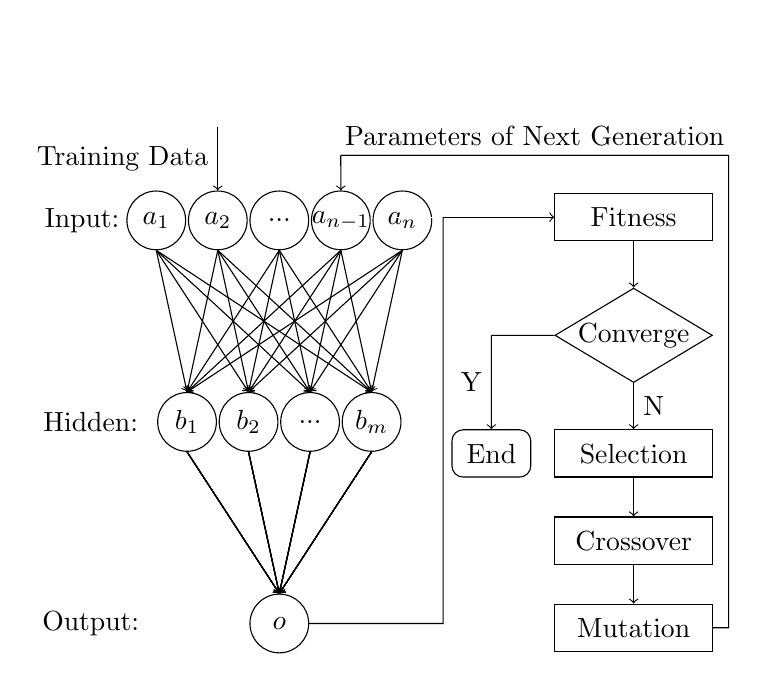
\begin{tikzpicture}
[ plain/.style={ draw=none, fill=none, }, remember picture, net/.style={ matrix of nodes, nodes={ draw, circle,
    inner sep=7.5pt
    },
  nodes in empty cells,
  column sep=-10.5pt,
  row sep=1.8cm
  }
]
    \draw[white] (2,4) rectangle (3,5);
%\draw[help lines] (-3cm,-6cm) grid (6cm,3cm);
\matrix[net] (mat)
{
              & |[plain]| &           & |[plain]|  &           & |[plain]| &           &  |[plain]|      &               \\
    |[plain]| &           & |[plain]| &            & |[plain]| &           & |[plain]| &                 & |[plain]|     \\ 
    |[plain]| & |[plain]| & |[plain]| & |[plain]|  &           & |[plain]| & |[plain]| &  |[plain]|      & |[plain]|     \\ 
  };

  \node at ($(mat-1-1.west)+(-16pt,0)$) {Input: };
  \node at ($(mat-2-2.west)+(-24pt,0)$) {Hidden:};
  \node at ($(mat-3-2.west)+(-24pt,0)$) {Output:};
  \node at (mat-1-1.base) {$a_1$};
  \node at (mat-1-3.base) {$a_2$};
  \node at (mat-1-5.base) {...};
  \node at (mat-1-7.base) {$a_{n-1}$};
  \node at (mat-1-9.base) {$a_{n}$};
  \node at (mat-2-2.base) {$b_1$};
  \node at (mat-2-4.base) {$b_2$};
  \node at (mat-2-6.base) {$...$};
  \node at (mat-2-8.base) {$b_{m}$};
  \node at (mat-3-5.base) {$o$};

 \foreach \a in {1,3,5,7,9}{
    \foreach \b in {2,4,6,8}{
        \draw[->] (mat-1-\a.south) -- (mat-2-\b.north);
     }
 \foreach \c in {2,4,6,8}
 \draw[->] (mat-2-\c.south) -- (mat-3-5.north);
  }
  
  % write text
  \draw[<-] (mat-1-3.north) -- +(0,0.8cm) node[pos=0.5,auto=left] {Training Data} ;
  \coordinate (shift) at (4.5,2.6);
  \begin{scope}[shift=(shift)]
    \tikzstyle{startstop} = [rectangle, rounded corners, minimum width=1.0cm,minimum height=0.6cm, text centered, draw=black]
    \tikzstyle{io} = [trapezium, trapezium left angle=70, trapezium right angle=110, minimum width=2cm, minimum height=0.6cm, text centered, draw=black]
    \tikzstyle{process} = [rectangle, minimum width=2cm, minimum height=0.6cm, text centered, draw=black]
    \tikzstyle{decision} = [diamond,minimum width=2cm, minimum height=1.2cm, draw=black]
    \node (fitness) [process] {Fitness};
    \node[yshift=-0.5cm] (decision) [decision, below of=fitness] {} node at (decision.base) {Converge};
    \node[yshift=-0.5cm] (selection) [process, below of=decision] {Selection};
    \node (crossover) [process] at ($(selection.south)+(0,-0.8cm)$) {Crossover};
    \node (mutation) [process] at ($(crossover.south)+(0,-0.8cm)$)  {Mutation};
    \node (end) [startstop] at ($(selection.west)+(-0.8cm,0cm)$) {End};

    \draw [->] (fitness) -- (decision);
    \draw [->] (decision.south) -- (selection.north) node[auto=left,pos=0.5]{N};
    \draw [->] (selection.south) -- (crossover.north);
    \draw [->] (crossover.south) -- (mutation.north);

    % draw intersection
    \draw [white] (decision.west) -- ++(-1.5cm,0) coordinate (A);
    \draw [white] (end.north) -- ++(0,3cm) coordinate (B);
    \draw[<-] (end.north) -- (intersection cs: first line={(decision.west)--(A)}, second line={(end.north)--(B)}) node[pos=0.5,auto=left] {Y} coordinate (C);
    \draw (decision.west) -- (C);
    % draw intersection
    \draw[white] (mat-3-5.east) -- ++(1.7cm,0) coordinate (D) -- ++(0,6cm) coordinate (E);
    \draw[white] (fitness.west) -- ++(-2cm,0) coordinate (F);
    \draw (mat-3-5.east) -- ++(1.7cm,0) -- (intersection cs: first line={(fitness.west)--(F)}, second line={(D)--(E)});
    \draw[<-] (fitness.west) -- (intersection cs: first line={(fitness.west)--(F)}, second line={(D)--(E)});
    % draw intersection
    \draw[white] (mutation.east) -- ++(0.2cm,0) -- ++(0,6cm) coordinate (G) -- ++(-6cm,0) coordinate (H);
    \draw[white] (mat-1-7.north) coordinate (I) -- ++(0,1cm) coordinate (J);
    \draw (mutation.east) -- ++(0.2cm,0) -- ++(0,6cm) -- (intersection cs: first line={(G)--(H)}, second line={(I)-- (J)}) coordinate (L);
    \draw (G) -- (L) node[pos=0.5,auto=right] {Parameters of Next Generation};
    \draw[<-] (mat-1-7.north) -- (L);
  \end{scope}

\end{tikzpicture}



\begin{tikzpicture}
    \tikzstyle{block} = [rectangle, text centered, draw=black,
    minimum width=1.3cm, minimum height=0.3cm]
    \draw[white] (4,0.8) rectangle (5,1.6);
    \node (input) [block] {\tiny input};
    \node (l1-1) [block] at ($(input.south)+(-1.4cm,-0.5cm)$) {};
    \node (l1-2) [block] at ($(input.south)+(0.0cm,-0.5cm)$) {};
    \node (l1-3) [block] at ($(input.south)+(1.4cm,-0.5cm)$) {};
    \node (l2-1) [block] at ($(l1-1.south)+(0cm,-0.5cm)$){};
    \node (l2-2) [block] at ($(l1-3.south)+(0cm,-0.5cm)$){};
    \node (l3-1) [block] at ($(l2-1.south)+(0cm,-0.5cm)$){};
    \node (l4-1) [block] at ($(l1-2.south)+(0cm,-1.7cm)$) {};
    \node (output) [block] at ($(l4-1.south)+(0cm,-0.4cm)$) {\tiny output};

    \draw[->] (input.south) -- (l1-1.north);
    \draw[->] (input.south) -- (l1-2.north);
    \draw[->] (input.south) -- (l1-3.north);
    \draw[->] (l1-1.south) -- (l2-1.north);
    \draw[->] (l4-1.south) -- (output.north);

    \draw[->] (l1-3.south) -- (l2-2.north);
    \draw[->] (l2-1.south) -- (l3-1.north);
    \draw[->] (l3-1.south) -- (l4-1.north);
    \draw[->] (l2-2.south) -- (l4-1.north);
    \draw[->] (l1-2.south) -- (l4-1.north);
\end{tikzpicture}

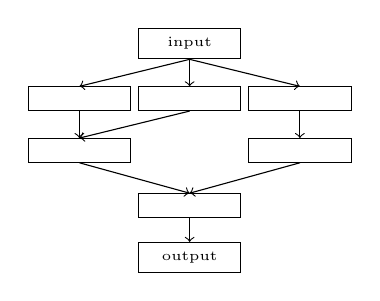
\begin{tikzpicture}
    \tikzstyle{block} = [rectangle, text centered, draw=black,
    minimum width=1.3cm, minimum height=0.3cm] 
    \node (input) [block] {\tiny input}; 
    \node (l1-1) [block] at ($(input.south)+(-1.4cm,-0.5cm)$) {};
    \node (l1-2) [block] at ($(input.south)+(0.0cm,-0.5cm)$) {};
    \node (l1-3) [block] at ($(input.south)+(1.4cm,-0.5cm)$) {};
    \node (l2-1) [block] at ($(l1-1.south)+(0cm,-0.5cm)$){};
    \node (l2-2) [block] at ($(l1-3.south)+(0cm,-0.5cm)$){};
    \node (l3-1) [block] at ($(l1-2.south)+(0cm,-1.2cm)$) {};
    \node (output) [block] at ($(l3-1.south)+(0cm,-0.5cm)$) {\tiny output};
    \draw[->] (input.south) -- (l1-1.north);

    \draw[->] (input.south) -- (l1-2.north);
    \draw[->] (input.south) -- (l1-3.north);
    \draw[->] (l1-1.south) -- (l2-1.north);
    \draw[->] (l1-2.south) -- (l2-1.north);
    \draw[->] (l1-3.south) -- (l2-2.north);
    \draw[->] (l2-1.south) -- (l3-1.north);
    \draw[->] (l2-2.south) -- (l3-1.north);

    \draw[->] (l3-1.south) -- (output.north);
\end{tikzpicture}

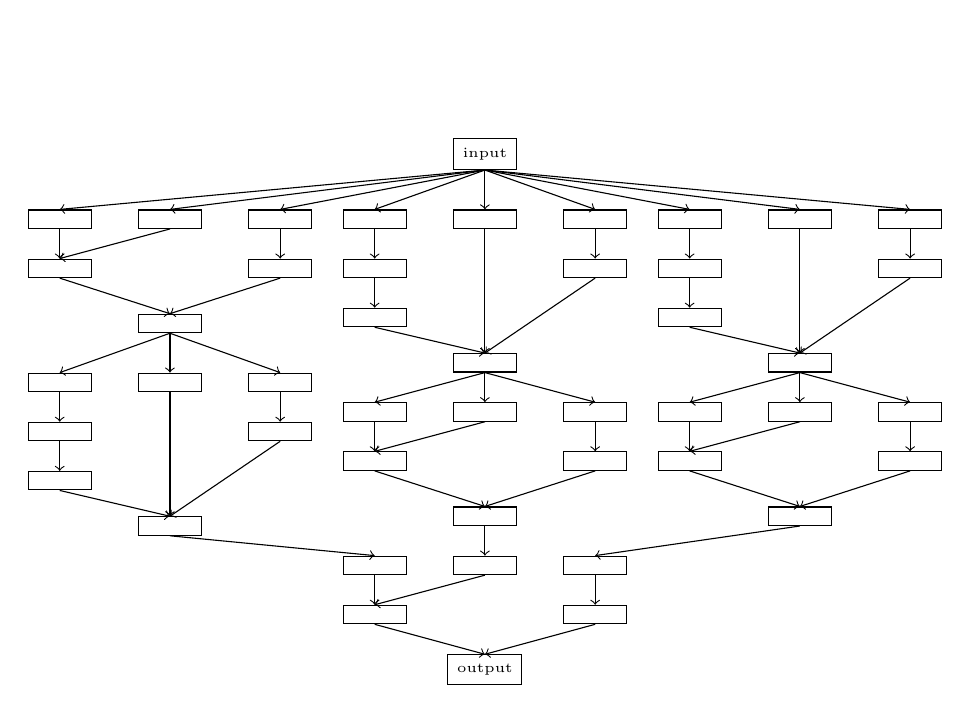
\begin{tikzpicture}
    \tikzstyle{block} = [rectangle, text centered, draw=black,
    minimum width=0.8cm, minimum height=0.22cm] 
    %\draw[help lines] (0,0) grid (4,5);
    \draw[white] (4,0.8) rectangle (5,1.6);

    \node (root) [block] {\tiny input}; 
    
    % first column, first layer
    \coordinate (shift) at ($(root.south)+(-4cm,-0.5cm)$);

    \begin{scope}[shift=(shift)]
    \node (input) [block,draw=white] {};
    \node (p1-l1-1) [block] at ($(input.south)+(-1.4cm,-0.0cm)$) {};
    \node (p1-l1-2) [block] at ($(input.south)+(0.0cm,-0.0cm)$) {};
    \node (p1-l1-3) [block] at ($(input.south)+(1.4cm,-0.0cm)$) {};
    \node (p1-l2-1) [block] at ($(p1-l1-1.south)+(0cm,-0.5cm)$){};
    \node (p1-l2-2) [block] at ($(p1-l1-3.south)+(0cm,-0.5cm)$){};
    \node (p1-l3-1-conn) [block] at ($(p1-l1-2.south)+(0cm,-1.2cm)$) {};

    \draw[->] (root.south) -- (p1-l1-1.north);
    \draw[->] (root.south) -- (p1-l1-2.north);
    \draw[->] (root.south) -- (p1-l1-3.north);
    \draw[->] (p1-l1-1.south) -- (p1-l2-1.north);
    \draw[->] (p1-l1-2.south) -- (p1-l2-1.north);

    \draw[->] (p1-l1-3.south) -- (p1-l2-2.north);
    \draw[->] (p1-l2-1.south) -- (p1-l3-1-conn.north);
    \draw[->] (p1-l2-2.south) -- (p1-l3-1-conn.north);
    \end{scope}

    % first column, second layer
    \coordinate (shift) at ($(p1-l3-1-conn.south)+(0cm,-0.5cm)$);

    \begin{scope}[shift=(shift)]
    \node (input) [block,draw=white] {};
    \node (p2-l1-1) [block] at ($(input.south)+(-1.4cm,-0.0cm)$) {};
    \node (p2-l1-2) [block] at ($(input.south)+(0.0cm,-0.0cm)$) {};
    \node (p2-l1-3) [block] at ($(input.south)+(1.4cm,-0.0cm)$) {};
    \node (p2-l2-1) [block] at ($(p2-l1-1.south)+(0cm,-0.5cm)$){};
    \node (p2-l2-2) [block] at ($(p2-l1-3.south)+(0cm,-0.5cm)$){};
    \node (p2-l3-1) [block] at ($(p2-l2-1.south)+(0cm,-0.5cm)$){};
    \node (c1-p2-l4-1) [block] at ($(p2-l1-2.south)+(0cm,-1.7cm)$) {};

    \draw[->] (p1-l3-1-conn.south) -- (p2-l1-1.north);
    \draw[->] (p1-l3-1-conn.south) -- (p2-l1-2.north);
    \draw[->] (p1-l3-1-conn.south) -- (p2-l1-3.north);
    \draw[->] (p2-l1-1.south) -- (p2-l2-1.north);

    \draw[->] (p2-l1-3.south) -- (p2-l2-2.north);
    \draw[->] (p2-l2-1.south) -- (p2-l3-1.north);
    \draw[->] (p2-l3-1.south) -- (c1-p2-l4-1.north);
    \draw[->] (p2-l2-2.south) -- (c1-p2-l4-1.north);
    \draw[->] (p2-l1-2.south) -- (c1-p2-l4-1.north);
        %%%%%%%%%%%%%%%%%%%%%%%%%
\end{scope}


    % second column, first layer
    \coordinate (shift) at ($(root.south)+(0cm,-0.5cm)$);

    \begin{scope}[shift=(shift)]
    \node (input) [block,draw=white] {};
    \node (p2-l1-1) [block] at ($(input.south)+(-1.4cm,-0.0cm)$) {};
    \node (p2-l1-2) [block] at ($(input.south)+(0.0cm,-0.0cm)$) {};
    \node (p2-l1-3) [block] at ($(input.south)+(1.4cm,-0.0cm)$) {};
    \node (p2-l2-1) [block] at ($(p2-l1-1.south)+(0cm,-0.5cm)$){};
    \node (p2-l2-2) [block] at ($(p2-l1-3.south)+(0cm,-0.5cm)$){};
    \node (p2-l3-1) [block] at ($(p2-l2-1.south)+(0cm,-0.5cm)$){};
    \node (p2-l4-1-conn) [block] at ($(p2-l1-2.south)+(0cm,-1.7cm)$) {};

    \draw[->] (root.south) -- (p2-l1-1.north);
    \draw[->] (root.south) -- (p2-l1-2.north);
    \draw[->] (root.south) -- (p2-l1-3.north);
    \draw[->] (p2-l1-1.south) -- (p2-l2-1.north);

    \draw[->] (p2-l1-3.south) -- (p2-l2-2.north);
    \draw[->] (p2-l2-1.south) -- (p2-l3-1.north);
    \draw[->] (p2-l3-1.south) -- (p2-l4-1-conn.north);
    \draw[->] (p2-l2-2.south) -- (p2-l4-1-conn.north);
    \draw[->] (p2-l1-2.south) -- (p2-l4-1-conn.north);
        %%%%%%%%%%%%%%%%%%%%%%%%%
\end{scope}
   % second column, second layer

    \coordinate (shift) at ($(p2-l4-1-conn)+(0cm,-0.5cm)$);

    \begin{scope}[shift=(shift)]
    \node (input) [block,draw=white] {};
    \node (p1-l1-1) [block] at ($(input.south)+(-1.4cm,-0.0cm)$) {};
    \node (p1-l1-2) [block] at ($(input.south)+(0.0cm,-0.0cm)$) {};
    \node (p1-l1-3) [block] at ($(input.south)+(1.4cm,-0.0cm)$) {};
    \node (p1-l2-1) [block] at ($(p1-l1-1.south)+(0cm,-0.5cm)$){};
    \node (p1-l2-2) [block] at ($(p1-l1-3.south)+(0cm,-0.5cm)$){};
    \node (c2-p1-l3-1) [block] at ($(p1-l1-2.south)+(0cm,-1.2cm)$) {};

    \draw[->] (p2-l4-1-conn.south) -- (p1-l1-1.north);
    \draw[->] (p2-l4-1-conn.south) -- (p1-l1-2.north);
    \draw[->] (p2-l4-1-conn.south) -- (p1-l1-3.north);
    \draw[->] (p1-l1-1.south) -- (p1-l2-1.north);
    \draw[->] (p1-l1-2.south) -- (p1-l2-1.north);

    \draw[->] (p1-l1-3.south) -- (p1-l2-2.north);
    \draw[->] (p1-l2-1.south) -- (c2-p1-l3-1.north);
    \draw[->] (p1-l2-2.south) -- (c2-p1-l3-1.north);
    \end{scope}




    % third column, third layer
    \coordinate (shift) at ($(root.south)+(4cm,-0.5cm)$);
    \begin{scope}[shift=(shift)]
        \node (input) [block,draw=white] {};

    \node (p3-l1-1) [block] at ($(input.south)+(-1.4cm,-0.0cm)$) {};
    \node (p3-l1-2) [block] at ($(input.south)+(0.0cm,-0.0cm)$) {};
    \node (p3-l1-3) [block] at ($(input.south)+(1.4cm,-0.0cm)$) {};
    \node (p3-l2-1) [block] at ($(p3-l1-1.south)+(0cm,-0.5cm)$){};
    \node (p3-l2-2) [block] at ($(p3-l1-3.south)+(0cm,-0.5cm)$){};
    \node (p3-l3-1) [block] at ($(p3-l2-1.south)+(0cm,-0.5cm)$){};
    \node (p3-l4-1-conn) [block] at ($(p3-l1-2.south)+(0cm,-1.7cm)$) {};

    \draw[->] (root.south) -- (p3-l1-1.north);
    \draw[->] (root.south) -- (p3-l1-2.north);
    \draw[->] (root.south) -- (p3-l1-3.north);
    \draw[->] (p3-l1-1.south) -- (p3-l2-1.north);

    \draw[->] (p3-l1-3.south) -- (p3-l2-2.north);
    \draw[->] (p3-l2-1.south) -- (p3-l3-1.north);
    \draw[->] (p3-l3-1.south) -- (p3-l4-1-conn.north);
    \draw[->] (p3-l2-2.south) -- (p3-l4-1-conn.north);
    \draw[->] (p3-l1-2.south) -- (p3-l4-1-conn.north);
    \end{scope}

    % third column, second layer
    \coordinate (shift) at ($(p3-l4-1-conn)+(0cm,-0.5cm)$);

    \begin{scope}[shift=(shift)]
    \node (input) [block,draw=white] {};
    \node (p1-l1-1) [block] at ($(input.south)+(-1.4cm,-0.0cm)$) {};
    \node (p1-l1-2) [block] at ($(input.south)+(0.0cm,-0.0cm)$) {};
    \node (p1-l1-3) [block] at ($(input.south)+(1.4cm,-0.0cm)$) {};
    \node (p1-l2-1) [block] at ($(p1-l1-1.south)+(0cm,-0.5cm)$){};
    \node (p1-l2-2) [block] at ($(p1-l1-3.south)+(0cm,-0.5cm)$){};
    \node (c3-p1-l3-1) [block] at ($(p1-l1-2.south)+(0cm,-1.2cm)$) {};

    \draw[->] (p3-l4-1-conn.south) -- (p1-l1-1.north);
    \draw[->] (p3-l4-1-conn.south) -- (p1-l1-2.north);
    \draw[->] (p3-l4-1-conn.south) -- (p1-l1-3.north);
    \draw[->] (p1-l1-1.south) -- (p1-l2-1.north);
    \draw[->] (p1-l1-2.south) -- (p1-l2-1.north);

    \draw[->] (p1-l1-3.south) -- (p1-l2-2.north);
    \draw[->] (p1-l2-1.south) -- (c3-p1-l3-1.north);
    \draw[->] (p1-l2-2.south) -- (c3-p1-l3-1.north);
    \end{scope}

   % second column, third layer
    \coordinate (shift) at ($(c2-p1-l3-1)+(0cm,-0.5cm)$);


    \begin{scope}[shift=(shift)]
    \node (input) [block,draw=white] {};
    \node (p1-l1-1) [block] at ($(input.south)+(-1.4cm,-0.0cm)$) {};
    \node (p1-l1-2) [block] at ($(input.south)+(0.0cm,-0.0cm)$) {};
    \node (p1-l1-3) [block] at ($(input.south)+(1.4cm,-0.0cm)$) {};
    \node (p1-l2-1) [block] at ($(p1-l1-1.south)+(0cm,-0.5cm)$){};
    \node (p1-l2-2) [block] at ($(p1-l1-3.south)+(0cm,-0.5cm)$){};
    \node (p1-l3-1) [block] at ($(p1-l1-2.south)+(0cm,-1.2cm)$) {\tiny output};

    \draw[->] (c1-p2-l4-1.south) -- (p1-l1-1.north);
    \draw[->] (c2-p1-l3-1.south) -- (p1-l1-2.north);
    \draw[->] (c3-p1-l3-1.south) -- (p1-l1-3.north);
    \draw[->] (p1-l1-1.south) -- (p1-l2-1.north);
    \draw[->] (p1-l1-2.south) -- (p1-l2-1.north);

    \draw[->] (p1-l1-3.south) -- (p1-l2-2.north);
    \draw[->] (p1-l2-1.south) -- (p1-l3-1.north);
    \draw[->] (p1-l2-2.south) -- (p1-l3-1.north);
    \end{scope}
\end{tikzpicture}
\begin{tikzpicture}
    \tikzstyle{block} = [rectangle, text centered, draw=black,
    minimum width=1.3cm, minimum height=0.3cm] 

    \draw[white] (4,0.8) rectangle (5,1.6);
    
    \node (input) [block] {\tiny input}; 
    \node (l1-1) [block] at ($(input.south)+(-1.4cm,-0.5cm)$) {};
    \node (l1-2) [block] at ($(input.south)+(0.0cm,-0.5cm)$) {}; \node (l1-3) [block] at ($(input.south)+(1.4cm,-0.5cm)$) {}; \node (l2-1) [block] at ($(l1-1.south)+(0cm,-0.5cm)$){}; \node (l2-2) [block] at ($(l1-3.south)+(0cm,-0.5cm)$){};
    \node (p1-connect-node) [block] at ($(l1-2.south)+(0cm,-1.2cm)$) {};

    \draw[->] (input.south) -- (l1-1.north);
    \draw[->] (input.south) -- (l1-2.north);
    \draw[->] (input.south) -- (l1-3.north);
    \draw[->] (l1-1.south) -- (l2-1.north);
    \draw[->] (l1-2.south) -- (l2-1.north);

    \draw[->] (l1-3.south) -- (l2-2.north);
    \draw[->] (l2-1.south) -- (l3-1.north);
    \draw[->] (l2-2.south) -- (p1-connect-node.north);

    \coordinate (shift) at ($(p1-connect-node.south)+(0cm,-0.5cm)$);

    \begin{scope}[shift=(shift)]
    \tikzstyle{block} = [rectangle, text centered, draw=black,
    minimum width=1.3cm, minimum height=0.3cm]
    \node (l1-1) [block] at ($(p1-connect-node.south)+(-1.4cm,-0.5cm)$) {};
    \node (l1-2) [block] at ($(p1-connect-node.south)+(0.0cm,-0.5cm)$) {};
    \node (l1-3) [block] at ($(p1-connect-node.south)+(1.4cm,-0.5cm)$) {};
    \node (l2-1) [block] at ($(l1-1.south)+(0cm,-0.5cm)$){};
    \node (l2-2) [block] at ($(l1-3.south)+(0cm,-0.5cm)$){};
    \node (l3-1) [block] at ($(l2-1.south)+(0cm,-0.5cm)$){};
    \node (p2-connect-node) [block] at ($(l1-2.south)+(0cm,-1.7cm)$) {};

    \draw[->] (p1-connect-node.south) -- (l1-1.north);
    \draw[->] (p1-connect-node.south) -- (l1-2.north);
    \draw[->] (p1-connect-node.south) -- (l1-3.north);
    \draw[->] (l1-1.south) -- (l2-1.north);

    \draw[->] (l1-3.south) -- (l2-2.north);
    \draw[->] (l2-1.south) -- (l3-1.north);
    \draw[->] (l3-1.south) -- (p2-connect-node.north);
    \draw[->] (l2-2.south) -- (p2-connect-node.north);
    \draw[->] (l1-2.south) -- (p2-connect-node.north);
    \end{scope}

    % third
    \coordinate (shift) at ($(p2-connect-node.south)+(0cm,-0.5cm)$);

    \begin{scope}[shift=(shift)]
    \tikzstyle{block} = [rectangle, text centered, draw=black,
    minimum width=1.3cm, minimum height=0.3cm] 
    \node (l1-1) [block] at ($(p2-connect-node.south)+(-1.4cm,-0.5cm)$) {};
    \node (l1-2) [block] at ($(p2-connect-node.south)+(0.0cm,-0.5cm)$) {};
    \node (l1-3) [block] at ($(p2-connect-node.south)+(1.4cm,-0.5cm)$) {};
    \node (l2-1) [block] at ($(l1-1.south)+(0cm,-0.5cm)$){};
    \node (l2-2) [block] at ($(l1-3.south)+(0cm,-0.5cm)$){};
    \node (l3-1) [block] at ($(l1-2.south)+(0cm,-1.2cm)$) {\tiny output};

    \draw[->] (p2-connect-node.south) -- (l1-1.north);
    \draw[->] (p2-connect-node.south) -- (l1-2.north);
    \draw[->] (p2-connect-node.south) -- (l1-3.north);
    \draw[->] (l1-1.south) -- (l2-1.north);
    \draw[->] (l1-2.south) -- (l2-1.north);

    \draw[->] (l1-3.south) -- (l2-2.north);
    \draw[->] (l2-1.south) -- (l3-1.north);
    \draw[->] (l2-2.south) -- (l3-1.north);
    \end{scope}
\end{tikzpicture}
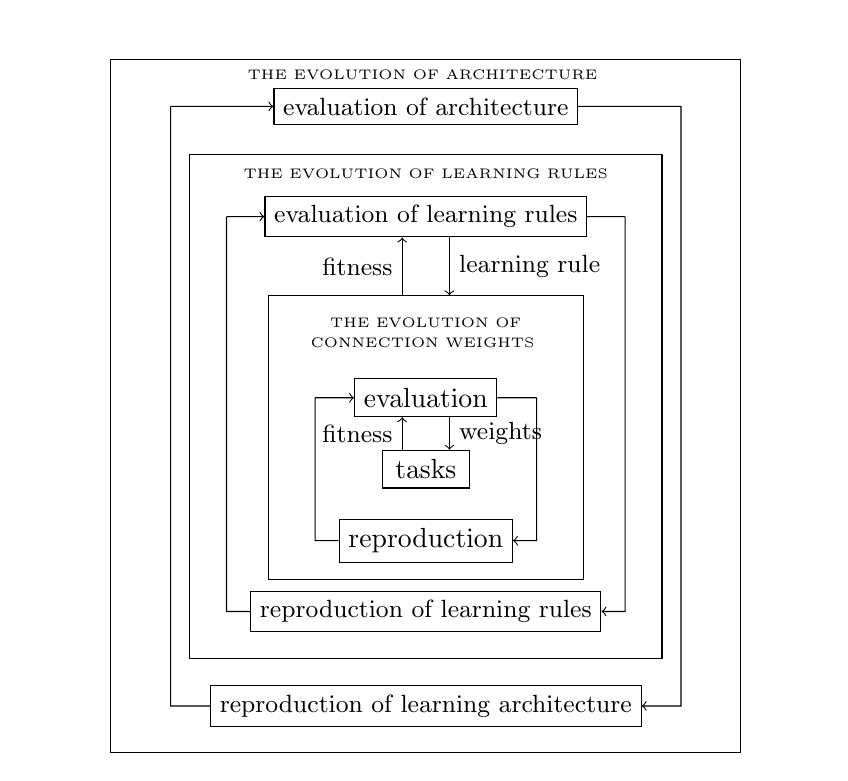
\begin{tikzpicture}
    %\draw[help lines] (-3cm,-6cm) grid (6cm, 6cm);
    \tikzstyle{block} = [rectangle, text centered, draw=black,
    minimum width=1.1cm, minimum height=0.4cm]
    \draw[white] (4,4.5) rectangle (5,5.6);
    
    % first level
    \node (evaluation-parent) [block, minimum width=2.6cm, minimum
        height=1.8cm,draw=white] {};
    \node (evaluation) [block] at ($(evaluation-parent.north)$) {evaluation};
    \node (reproduction) [block] at ($(evaluation-parent.south)$) {reproduction};
    \node (tasks) [block, minimum width=1.1cm, minimum height=0.4cm] {tasks};


    \draw[->] ($(evaluation.south)+(0.3cm,0cm)$) --
        ($(tasks.north)+(0.3cm,0cm)$) node[auto=left, pos=0.5] {\small weights}; 
    \draw[<-] ($(evaluation.south)+(-0.3cm,0cm)$) --
        ($(tasks.north)+(-0.3cm,0cm)$) node[auto=right, pos=0.5] {\small fitness}; 

    % get intersection
    \draw[white] (evaluation.west) coordinate (A) -- ++(-3cm,0) coordinate (B);
    \draw[white] (reproduction.west) -- ++(-0.3cm,0) coordinate (C) -- ++(0,4cm) coordinate
        (D);
    \draw[black] (reproduction.west) -- ++(-0.3cm,0) -- (intersection cs:
        first line={(A)--(B)}, second line={(C)--(D)}) coordinate (E);
    \draw[->] (E) -- (evaluation.west);

    \draw[white] (evaluation.east) coordinate (E) -- ++(2cm,0) coordinate (F);
    \draw[white] (reproduction.east) -- ++(0.3cm,0) coordinate (G) -- ++(0,4cm) coordinate
        (H);
    \draw[<-] (reproduction.east) -- ++(0.3cm,0) -- (intersection cs:
        first line={(E)--(F)}, second line={(G)--(H)}) coordinate (I);
    \draw (I) -- (evaluation.east);

    % second level
    \node (level2) [block, minimum width=4.0cm, minimum height=3.6cm] at
        (0cm,0.4cm) {};
    \node [align=left] at ($(level2.north)+(0,-0.35cm)$) {\tiny THE EVOLUTION
        OF};
    \node [align=left] at ($(level2.north)+(0,-0.6cm)$) {\tiny CONNECTION
            WEIGHTS 
        };
    % third level
    \node (level3-assister) [block, draw=white, minimum width=5cm, minimum height=5cm] at
        (0, 0.7cm)  {};
    \node (evaluation) [block] at ($(level3-assister.north)$) {\small evaluation of
        learning rules};
    \node (reproduction) [block] at ($(level3-assister.south)$) {\small reproduction of
        learning rules};

    \draw[->] ($(evaluation.south)+(0.3cm,0cm)$) --
        ($(level2.north)+(0.3cm,0cm)$) node[auto=left, pos=0.5] {\small learning
        rule}; 
    \draw[<-] ($(evaluation.south)+(-0.3cm,0cm)$) --
        ($(level2.north)+(-0.3cm,0cm)$) node[auto=right, pos=0.5] {\small fitness}; 

    \draw[white] (evaluation.west) coordinate (A) -- ++(-3cm,0) coordinate (B);
    \draw[white] (reproduction.west) -- ++(-0.3cm,0) coordinate (C) -- ++(0,4cm) coordinate
        (D);
    \draw[black] (reproduction.west) -- ++(-0.3cm,0) -- (intersection cs:
        first line={(A)--(B)}, second line={(C)--(D)}) coordinate (E);
    \draw[->] (E) -- (evaluation.west);

    \draw[white] (evaluation.east) coordinate (E) -- ++(2cm,0) coordinate (F);
    \draw[white] (reproduction.east) -- ++(0.3cm,0) coordinate (G) -- ++(0,4cm) coordinate
        (H);
    \draw[<-] (reproduction.east) -- ++(0.3cm,0) -- (intersection cs:
        first line={(E)--(F)}, second line={(G)--(H)}) coordinate (I);
    \draw (I) -- (evaluation.east);
   % fourth level
    \node (level4) [block, minimum width=6cm, minimum
        height=6.4cm] at
        (0, 0.8cm)  {};
    \node [align=left] at ($(level4.north)+(0,-0.25cm)$) {\tiny THE EVOLUTION
        OF LEARNING RULES};
    % level five
    \node (level5-assister) [block, draw=white, minimum width=8.4cm, minimum
        height=7.6cm] at
        (0, 0.8cm)  {};
    \node (evaluation) [block] at ($(level5-assister.north)$) {\small evaluation of
        architecture};
    \node (reproduction) [block] at ($(level5-assister.south)$) {\small reproduction of
        learning architecture};

    \draw[white] (evaluation.west) coordinate (A) -- ++(-3cm,0) coordinate (B);
    \draw[white] (reproduction.west) -- ++(-0.5cm,0) coordinate (C) -- ++(0,4cm) coordinate
        (D);
    \draw[black] (reproduction.west) -- ++(-0.5cm,0) -- (intersection cs:
        first line={(A)--(B)}, second line={(C)--(D)}) coordinate (E);
    \draw[->] (E) -- (evaluation.west);

    \draw[white] (evaluation.east) coordinate (E) -- ++(2cm,0) coordinate (F);
    \draw[white] (reproduction.east) -- ++(0.5cm,0) coordinate (G) -- ++(0,4cm) coordinate
        (H);
    \draw[<-] (reproduction.east) -- ++(0.5cm,0) -- (intersection cs:
        first line={(E)--(F)}, second line={(G)--(H)}) coordinate (I);
    \draw (I) -- (evaluation.east);
    % level 6
    \node (level6) [block, minimum width=8.0cm, minimum
        height=8.8cm] at
        (0, 0.8cm)  {};
    \node [align=left] at ($(level6.north)+(0,-0.2cm)$) {\tiny THE EVOLUTION OF
            ARCHITECTURE
        };
\end{tikzpicture}
\begin{comment}
\end{comment}
\end{document}
